%!TEX TS-program = xelatex
\documentclass[]{friggeri-cv}
\usepackage{afterpage}
\usepackage{hyperref}
\usepackage{color}
\usepackage{xcolor}
\usepackage{fontspec}
\usepackage[utf8]{inputenc}

\hypersetup{
    pdftitle={},
    pdfauthor={},
    pdfsubject={},
    pdfkeywords={},
    colorlinks=false,           % no lik border color
    allbordercolors=white       % white border color for all
}

\RequirePackage{xcolor}
\definecolor{pblue}{HTML}{0395DE}

\begin{document}

\begin{figure}[!h]
	\begin{minipage}{0.48\textwidth}
		\begin{flushleft}
			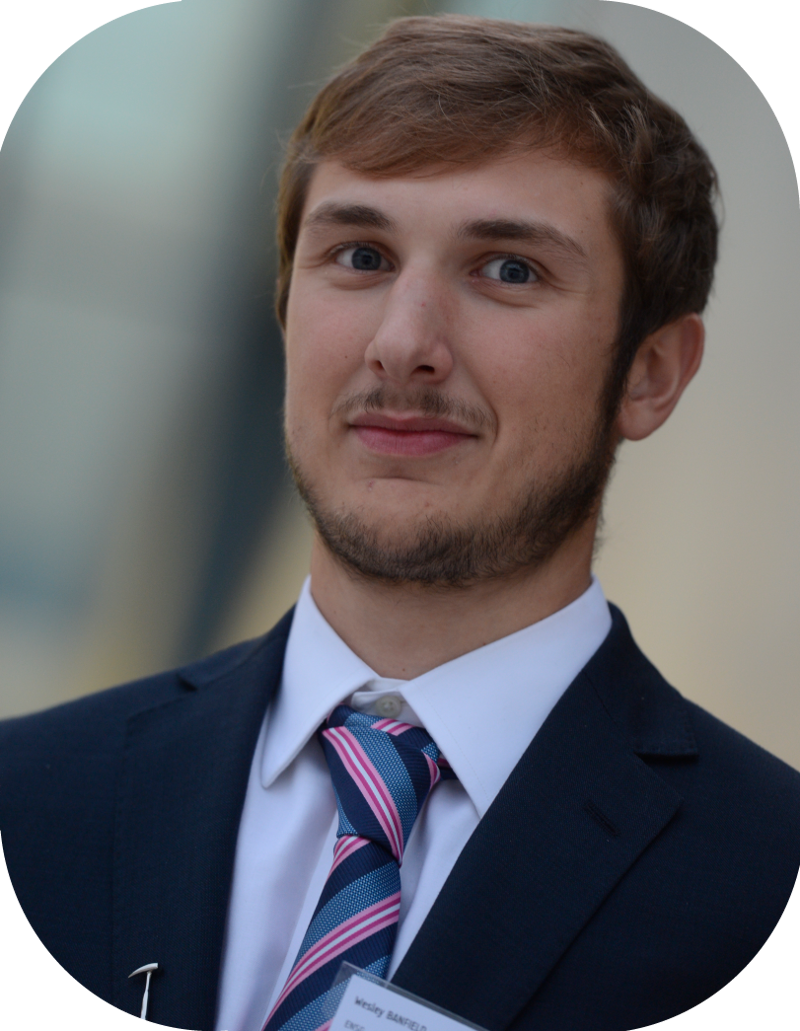
\includegraphics[width=2.75cm]{img/profile.png}
		\end{flushleft}
	\end{minipage}\hfill
	\header{Wesley}{ Banfield}
 	{Unconventional Thinker - Geologist - Software Engineer}
	\begin{minipage}{0.48\textwidth}
		\begin{flushright}
			
\includegraphics[width=2.75cm]{img/QR.png}
		\end{flushright}
	\end{minipage}
\end{figure}
\vspace{-0.75cm}
% Fake text to add separator      
\fcolorbox{white}{gray}{\parbox{\dimexpr\textwidth-2\fboxsep-2\fboxrule}{%
.....
}}

\begin{quote}
\large
Disruption occurs when you are not paying attention, staying at the forefront of innovation is key. Oil \& Gas Geologist by trade with a specialization in Software Engineering I strive to \textbf{unite technology and innovation} to push the boundaries of what’s possible.
\end{quote}

\begin{center}
\vspace{6pt}
\href{mailto:wesleybanfield@gmail.com}{\textbf{wesleybanfield@gmail.com}}
\\+64 27 777 55 09, Christchurch, New Zealand
\\\emph{GB, USA citizen, FR bilingual}
\vspace{3pt}
\\\href{https://www.linkedin.com/in/wesleybanfield/}{LinkedIn},
\href{https://github.com/WesleyTheGeolien}{GitHub}
\end{center}

\vspace{6pt}
\begin{table}[!h]
	\centering
	\begin{tabular}{L{3.25cm}cL{2cm}L{2.25cm}cL{2cm}L{2.25cm}c}
		\multicolumn{2}{c}{\large\textbf{\textcolor{pblue}{Technologies}}} && \multicolumn{2}{c}{\large\textbf{\textcolor{pblue}{Languages}}} && \multicolumn{2}{c}{\large\textbf{\textcolor{pblue}{Geological Software}}} \\
		\textbf{Jupyter} & 
\includegraphics[scale=0.40]{img/4stars.png} && \textbf{Python} & 
\includegraphics[scale=0.40]{img/5stars.png} && \textbf{Leapfrog} & 
\includegraphics[scale=0.40]{img/5stars.png} \\
		\textbf{Orange} &  
\includegraphics[scale=0.40]{img/4stars.png} &&
		\textbf{C++} & 
\includegraphics[scale=0.4]{img/3stars.png} &&
		\href{http://www.ccgalberta.com/}{\textbf{CCG}} & 
\includegraphics[scale=0.40]{img/5stars.png} \\
		\textbf{Plotly/Dash} & 
\includegraphics[scale=0.40]{img/4stars.png} &&
		\textbf{\LaTeX} & 
\includegraphics[scale=0.4]{img/4stars.png} &&
		\href{http://www.pdgm.com/products/skua-gocad/}{\textbf{Skua}} & 
\includegraphics[scale=0.40]{img/3stars.png} \\
		\textbf{Docker} & 
\includegraphics[scale=0.40]{img/3stars.png} && 
		& 
		&&
		\textbf{QGis} & 
\includegraphics[scale=0.40]{img/3stars.png} \\
		\textbf{Sklearn}&
		
\includegraphics[scale=0.40]{img/3stars.png} &&
		&
		&&
		\href{https://snowdengroup.com/software/supervisor/}{\textbf{Supervisor}}&
		
\includegraphics[scale=0.40]{img/3stars.png}\\
		\textbf{Microsoft PowerApps / Flow}&
		
\includegraphics[scale=0.40]{img/2stars.png}&&
		&
		&&
		&
	\end{tabular}
\end{table}

\section{Experience}
\begin{entrylist}
  \entry
    {01/17 - 05/19}
    {Research Engineer}
    {\href{https://www.seequent.com/}{Seequent, Christchurch New Zealand}}
    {I pride myself on thinking laterally and outside of the box to provide novel innovative solutions, drawing on insights from both my geological and software engineering backgrounds.
    \\[3pt]
    The role permitted vast exposure to the company and clients. Regular client meetings and presentations were held as well as working, and leading, interdisciplinary initiatives.
    \\[3pt]
    Seequent are the developpers of the \href{https://www.leapfrog3d.com/}{Leapfrog Suite}, a world standard for 3D implicit geological modelling software. Daily use and technical insights led me to become an expert user, continuously pushing the limits.
    \\[6pt]
   	\textbf{New Technologies} Some problems call for thinking outside the box and implementing new technologies from the base up. Examples of these projects included web based dashboard creation, integration of Jupyter into workflows and deploying compute intensive tasks to the cloud.
   	\\[6pt]
   	\textbf{New Solutions} Other projects included the reuse of core IP in novel manners. For example the automated creation of geological models from sub sets of data to sample geological uncertainty. This work was presented at Seequent's \href{https://www.youtube.com/watch?v=jt26J5ljlA0}{Perth Lyceum}.
    \\[6pt]
   	\textbf{Core Strategy} Providing technical support for key business decisions including full verification of geostatistical implementations and creation of infrastructure to obtain and analyse usage metrics of Leapfrog software. 
    \\
    Reference : \href{mailto:tim.schurr@seequent.com}{Tim Schurr, Solutions Architect}
	}
  \entry
    {05/16 - 19/16}
    {Software Integration Engineering Internship}
    {\href{https://www.total.com/en}{Total, Pau France}}
    {Discretization plays an important part in coupled Oil \& Gas basin modelling. Too fine, the computation time prevails, too coarse and the calculations do not converge. As a software integration engineer I implemented an interface with the \href{http://www.ring-team.org/software/ringmesh}{RINGMesh} library to dynamically re-mesh during simulations.\\ Reference : \href{mailto:tristan.cornu@total.com}{Tristan Cornu, Pore pressure and Rock Mechanics Specialist}}
    \end{entrylist}
    
    \vspace*{\fill}
    \begin{entrylist}
    \entry
    {02/16 - 05/16}
    {Research Intern}
    {\href{http://www.ring-team.org/}{Ring Research Lab, Nancy France }}
    {Research and implementation of different automatic simultaneous well log correlation algorithms and creation of a SKUA-Gocad plug-in. The master's thesis was carried out in the lab that orginally developed SKUA-Gocad before commercialisation by Paradigm. The work was presented and published in the 2016 Ring Meeting. \\Reference : \href{mailto:Guillaume.Caumon@ensg.univ-lorraine.fr}{Dr. Guillaume Caumon, Head of Research team}}
    \entry
    {06/15 - 09/15}
    {Software Engineering Internship}
    {\href{https://www.seequent.com/}{Seequent, Christchurch New Zealand}}
    {Design and development of a graphical user interface for geostatistical analysis in Leapfrog 3D Geological modelling suite, later integrated into Leapfrog EDGE. Implementation of different geostatistical algorithms.
    \\
    Reference : \href{mailto:tim.mclennan@seequent.com}{Tim McLennan}}

	\entry
	{09/14 - 05/15}
	{Lab Research Project}
	{\href{http://georessources.univ-lorraine.fr/}{GeoRessources, Nancy France}}
	{Geochemistry can be used to date oil, however when in contact with water certain couples reset. The goal of the project was to develop an experimental protocol to analyse the behaviour of the Rhenium / Osmium couple. Automated graphing tools where developed to analyse the ICP-MS results.
		\\
		Reference : Raymond Michels}
\end{entrylist}
\section{Education MEng, MSc}
\begin{entrylist}
  \entry
    {2013 - 2016}
    {Master in Geological Engineering with specialisation in Numerical Geology and Oil \& Gas Engineering}
    {\href{http://ensg.univ-lorraine.fr/english/}{French National School of Geological Engineering}}
    {\emph{Ecole Nationale Superieure de Geologie} is a leading French engineering school specialising in geosciences and delivering an Engineering diploma combined with a Master from the University of Lorraine.\\ \emph{Curriculum}: Oil and Gas Engineering and Numerical Geology\\ 
    \emph{Main subjects}:  Software Development, Interface Design, Computer Geometry, Visualisation and Parallelism, Mathematical concepts of geomodelling, Finite Elements, Structural Geology, Petroleum Systems, Sedimentology, Geomechanics.\\
    \emph{Title of Thesis}: ”Current automatic well log correlation techniques, their advantages and drawbacks”.
    \emph{References}: Dr. Guillaume Caumon, Jonathan Edwards\\}
  \entry
    {2011 - 2013}
    {\href{https://en.wikipedia.org/wiki/Classe_preparatoire_aux_grandes_ecoles}{Classes Preparatoires aux Grandes Ecoles}}
    {Lycee Pierre de Fermat, Toulouse France}
    {2 years of intensive general scientific courses before national exams for entry to the French Grandes Ecoles, carried out at Pierre de Fermat, one of the top preparatory schools finishing in the top 10\% nationally.\\ 
    \emph{Main subjects}: Mathematics, Physics, Chemistry, Biology and Geology, \\}
\end{entrylist}
\vspace*{\fill}

\end{document}
